\section*{Q6}

Similarly to the non-reordering decoder, increases in the number of
translations $k$ lead to major improvements at first, but fewer improvements
$k>50$. In contrast to the results obtained from the simple decoder,
increases in the stack size $s$ do not fade out as quickly. The changes also
have a larger effect for smaller $s$, with the biggest difference between
$s=1$ and $s=2$. Even in the reordering decoder, we do not observe any
performance increases for $s>20$.

We note that $k$ and $s$ have a much larger effect on runtime than they have
for the simple decoder. Nonetheless, the run times of both decoders are in
the same order of magnitude (see Fig.~\ref{swaptime}). For $k = s = 10$, the
sentences are relatively well-formed, though still difficult to understand.
Since we are still using a bigram model, it is not surprising that long-term
dependencies are not correctly resolved.

\begin{figure}
	\centering
	\begin{subfigure}{.8\linewidth}
		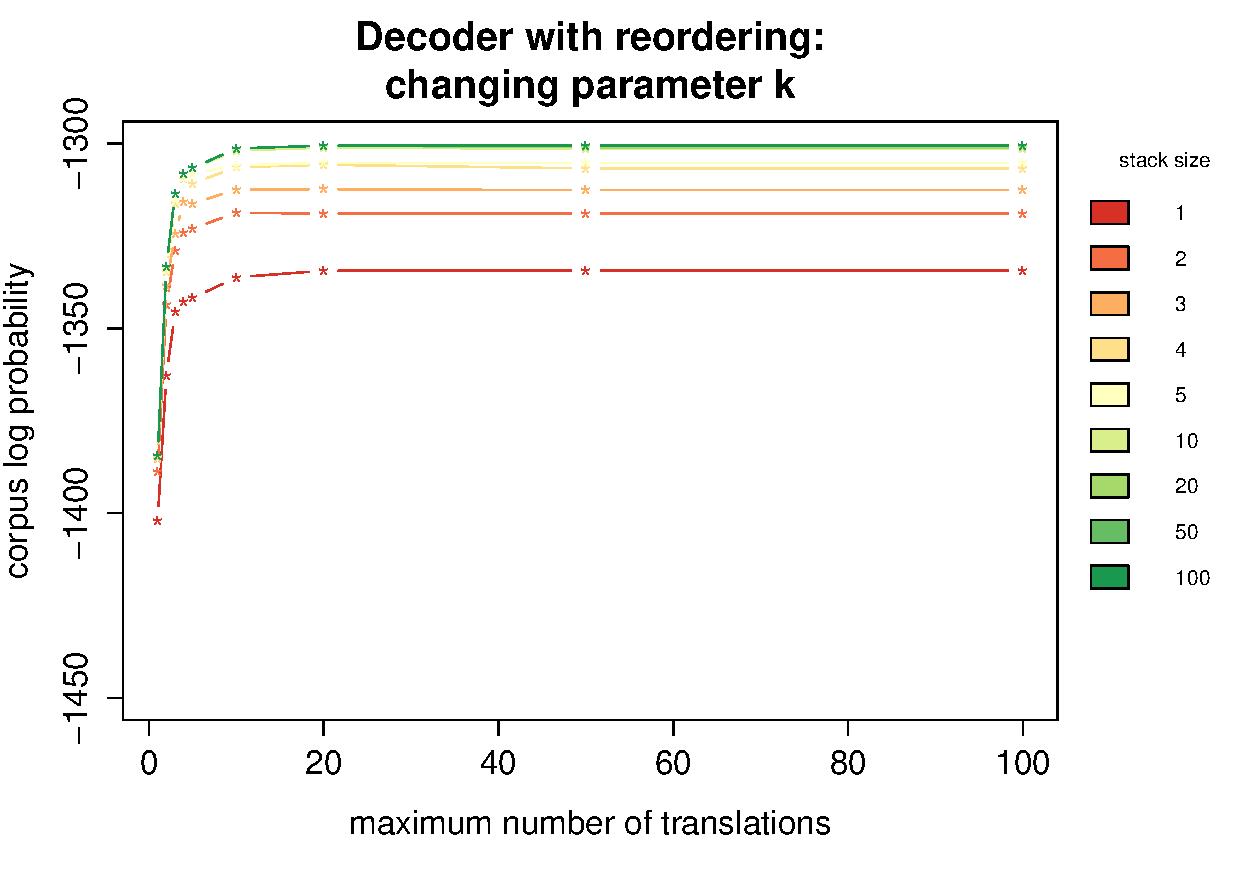
\includegraphics[scale=.65]{figures/d2_k.pdf}
		\caption{Increasing maximum number of translations, range [1--100].}
	\end{subfigure}
	\hskip2em
	\begin{subfigure}{.8\linewidth}
		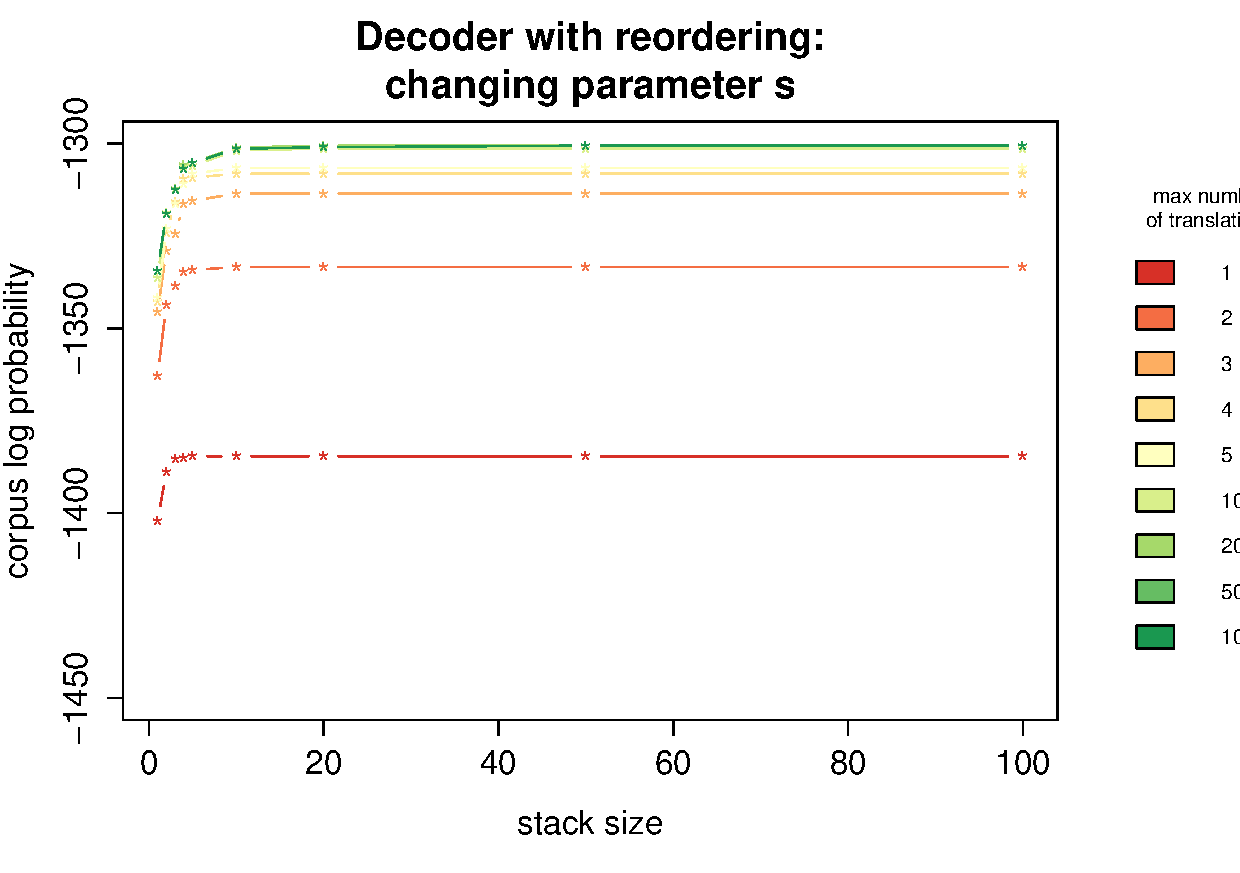
\includegraphics[scale=.65]{figures/d2_s.pdf}
		\caption{Increasing stack size, range [1--100].}
	\end{subfigure}
    \caption{Performance of decoder with local reordering.}\label{swap}
\end{figure}

\begin{figure}
	\centering
	\begin{subfigure}{.45\linewidth}
		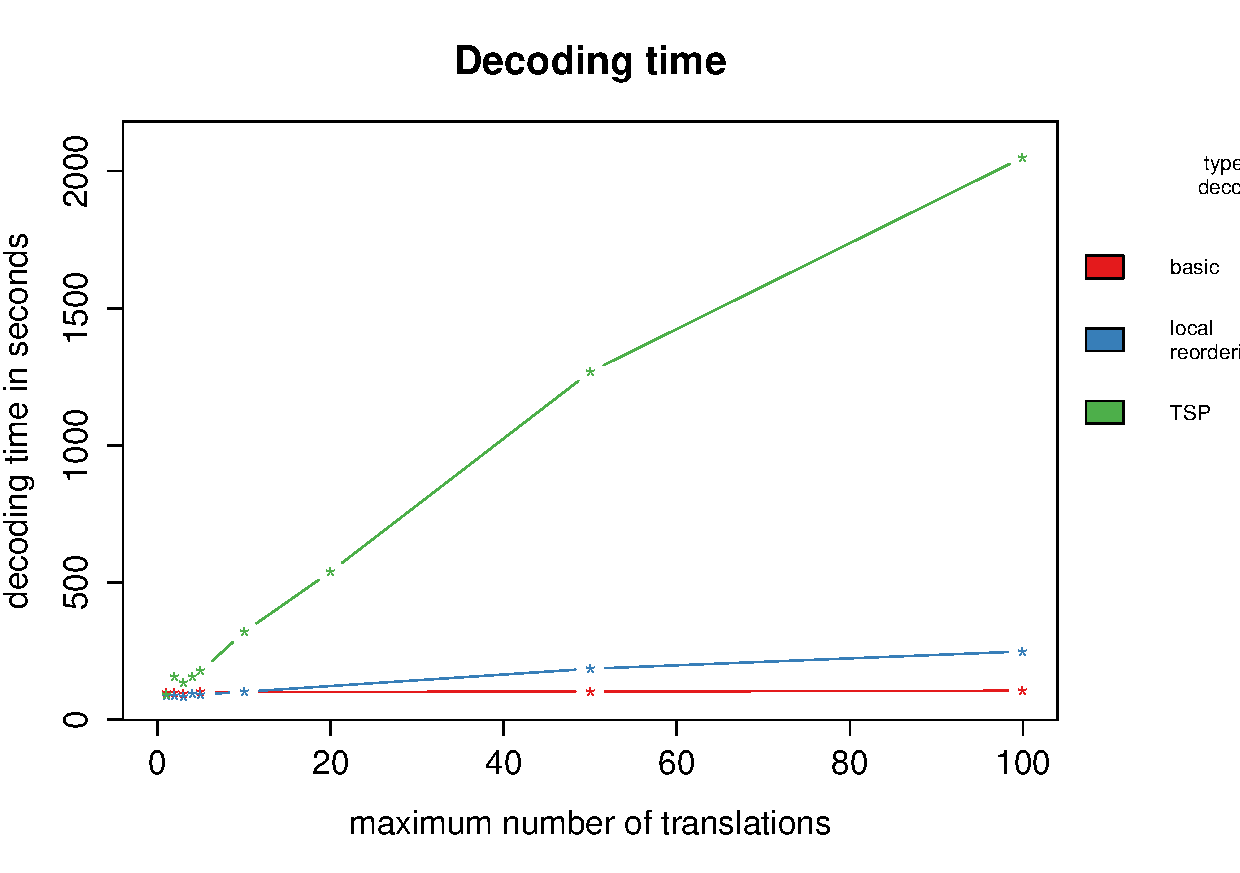
\includegraphics[scale=.35]{figures/time.pdf}
		\caption{Decoding time as function of maximum number of translations.}
	\end{subfigure}
	\hskip2em
	\begin{subfigure}{.45\linewidth}
		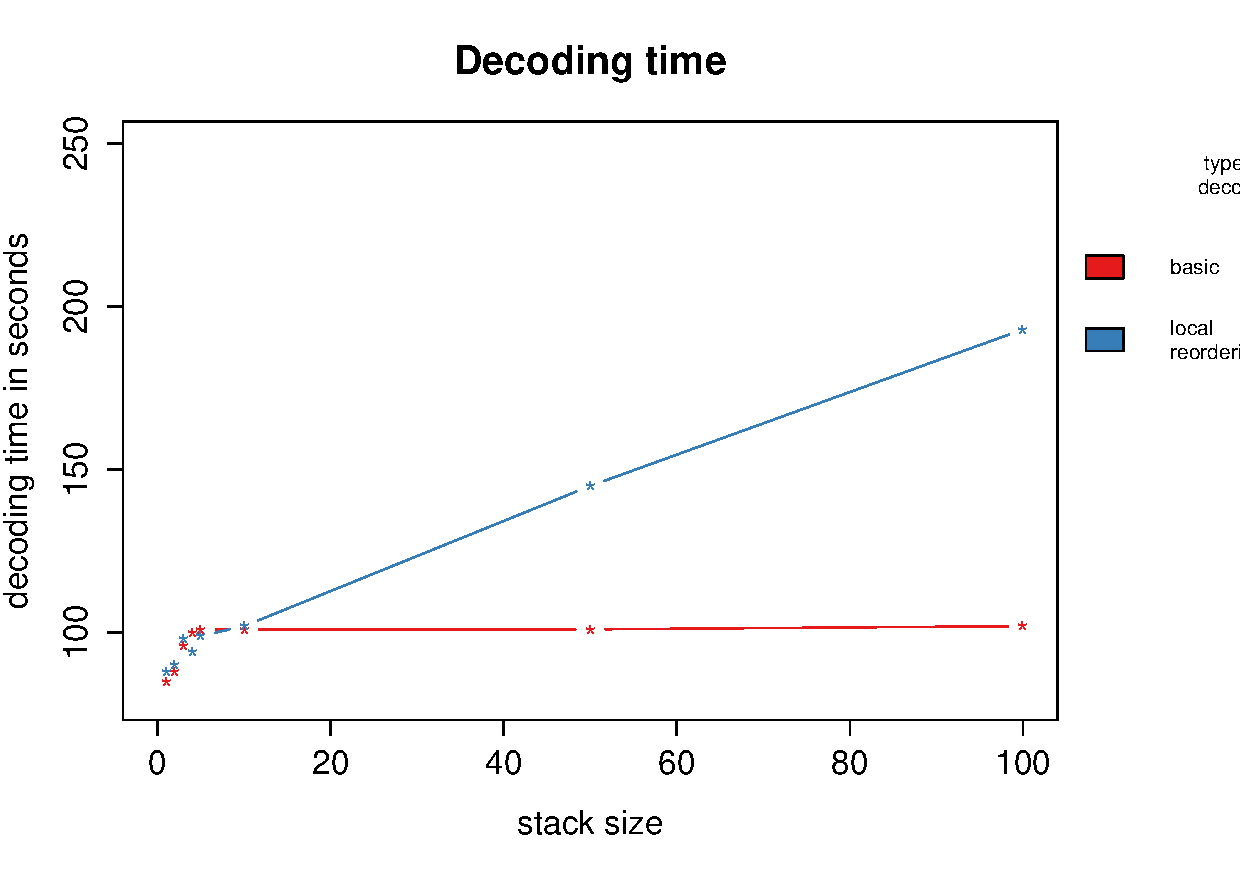
\includegraphics[scale=.35]{figures/time_d1_d2.pdf}
		\caption{Decoding time as a function of stack size.}
	\end{subfigure}
	\caption{Decoding time for the three decoders.}\label{swaptime}
\end{figure}

